\begin{figure}[h]
\centering
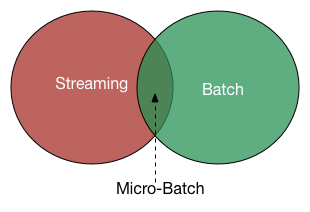
\includegraphics[width=0.35\textwidth]{eps/streambatch}
\caption{Conceptual view of micro-batching}
\label{fig_micro_batch}
\end{figure}







\section{Evaluation}
\label{eval}
\subsection{Configuration}
The following configurations are used throughput experiments:
\begin{itemize}
\item Cluster size: 2,3,4 and 8 node clusters
\item Parallelism within single node: number of cores, which is 16.
\item Parallelism within cluster: (Parallelism within single node) * (number of nodes)

\item Backpressure: enabled in all systems
\item Network bandwidth: 1Gb
\item Number of Data Engines running in parallel: 16
\item Allocated memory: 16GB
\item Cluster type: Standalone
\item Input size for aggregation use case: 150M * 16
\item Input size for join use case: 
\item Spark batch size: 4 seconds and 2 seconds
\item Window type: Processing time
\item Number of distinct keys in input: 160
\item Join inputs selectivity: 
\item $c_{a}$, acceptable queue limit: 1M
\item $c_{b}$ backpressure tolerated queue limit: 15M
\end{itemize}

\subsection{Keyed Windowed Aggregations}

\subsubsection{Storm}


\begin{figure*}
    \centering
    \begin{subfigure}[b]{0.49\textwidth}
        \includegraphics[width=\textwidth]{storm/2_1}
        \caption{2 Node latency histogram}
        \label{fig_no_queue}
    \end{subfigure}
    ~ %add desired spacing between images, e. g. ~, \quad, \qquad, \hfill etc. 
      %(or a blank line to force the subfigure onto a new line)
    \begin{subfigure}[b]{0.49\textwidth}
        \includegraphics[width=\textwidth]{storm/3_1}
        \caption{3 Node latency histogram}
        \label{fig_yes_queue}
    \end{subfigure}
    ~ %add desired spacing between images, e. g. ~, \quad, \qquad, \hfill etc. 
    %(or a blank line to force the subfigure onto a new line)
    \begin{subfigure}[b]{0.49\textwidth}
        \includegraphics[width=\textwidth]{storm/4_1}
        \caption{4 Node latency histogram}
        \label{fig_partial_queue}
    \end{subfigure}
        \begin{subfigure}[b]{0.49\textwidth}
        \includegraphics[width=\textwidth]{storm/8_1}
        \caption{8 Node latency histogram}
        \label{fig_partial_queue}
    \end{subfigure}


    \begin{subfigure}[b]{0.49\textwidth}
        \includegraphics[width=\textwidth]{storm/2_2}
        \caption{2 Node latency time series}
        \label{fig_no_queue}
    \end{subfigure}
    ~ %add desired spacing between images, e. g. ~, \quad, \qquad, \hfill etc. 
      %(or a blank line to force the subfigure onto a new line)
    \begin{subfigure}[b]{0.49\textwidth}
        \includegraphics[width=\textwidth]{storm/3_2}
        \caption{3 Node latency time series}
        \label{fig_yes_queue}
    \end{subfigure}
    ~ %add desired spacing between images, e. g. ~, \quad, \qquad, \hfill etc. 
    %(or a blank line to force the subfigure onto a new line)
    \begin{subfigure}[b]{0.49\textwidth}
        \includegraphics[width=\textwidth]{storm/4_2}
        \caption{4 Node latency time series}
        \label{fig_partial_queue}
    \end{subfigure}
        \begin{subfigure}[b]{0.49\textwidth}
        \includegraphics[width=\textwidth]{storm/8_2}
        \caption{8 Node latency time series}
        \label{fig_partial_queue}
    \end{subfigure}

    \label{fig_flink_agg_1}
        \caption{Latency of windowed aggregations for Storm}
\end{figure*}


\subsubsection{Spark}



\begin{figure*}
    \centering
    \begin{subfigure}[b]{0.49\textwidth}
        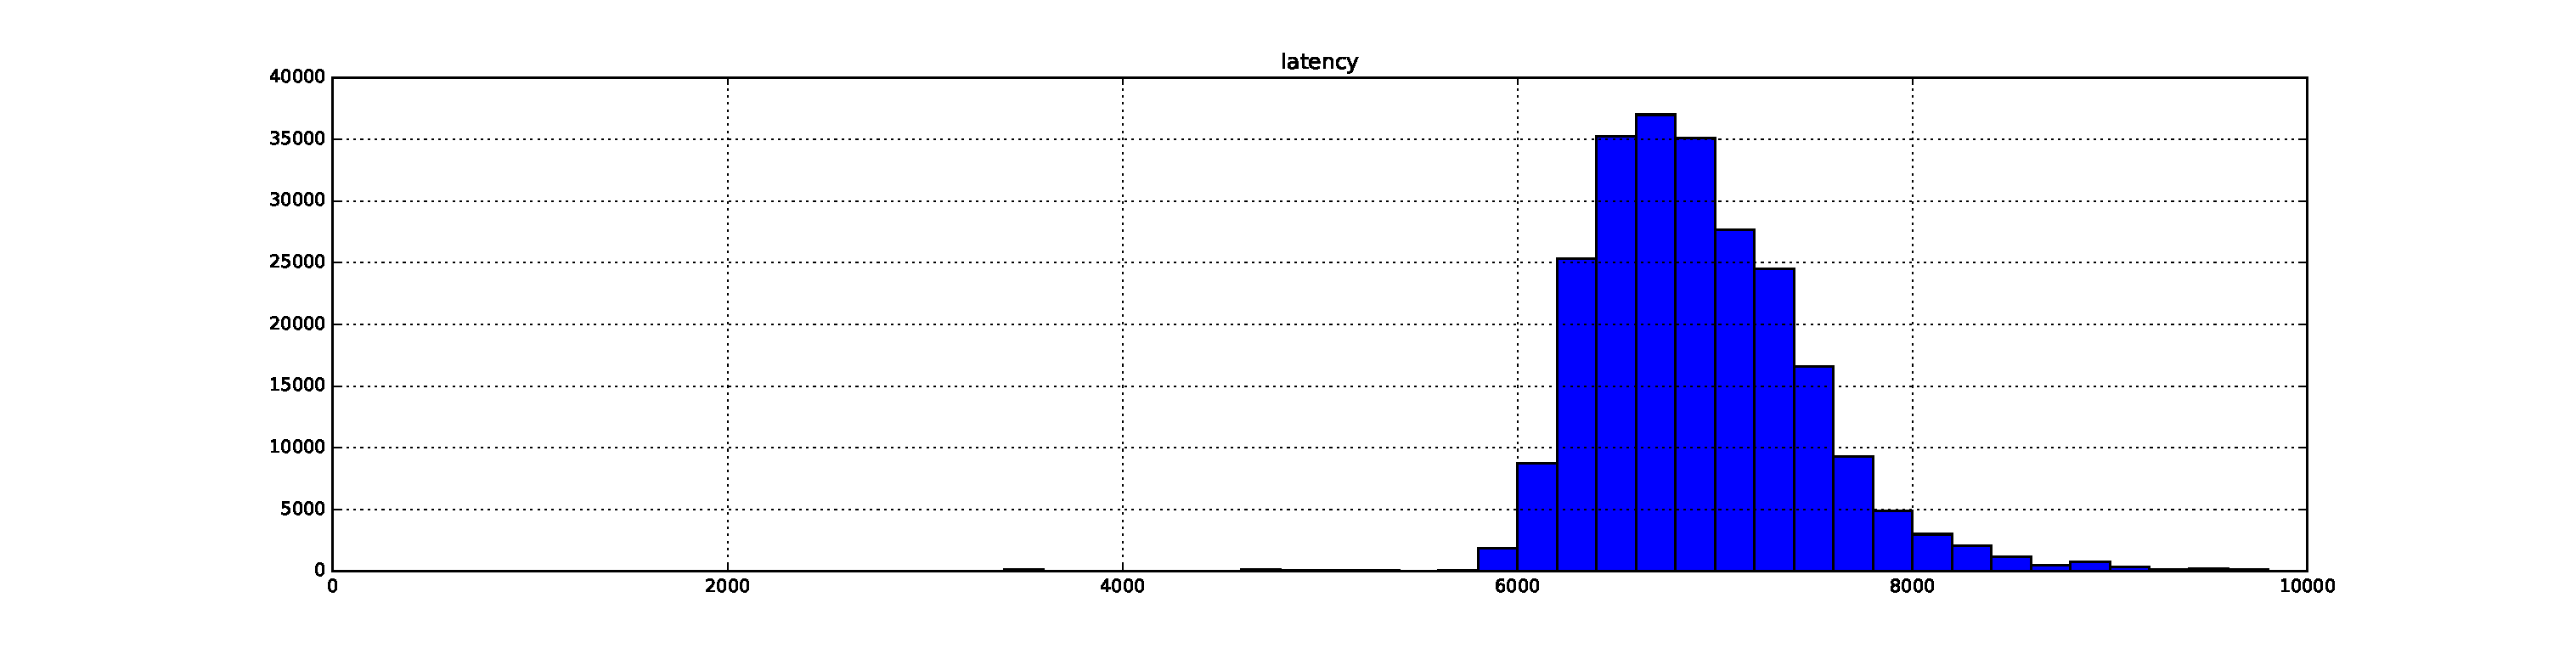
\includegraphics[width=\textwidth]{spark/2_4_1}
        \caption{2 Node latency histogram}
        \label{fig_no_queue}
    \end{subfigure}
    ~ %add desired spacing between images, e. g. ~, \quad, \qquad, \hfill etc. 
      %(or a blank line to force the subfigure onto a new line)
    \begin{subfigure}[b]{0.49\textwidth}
        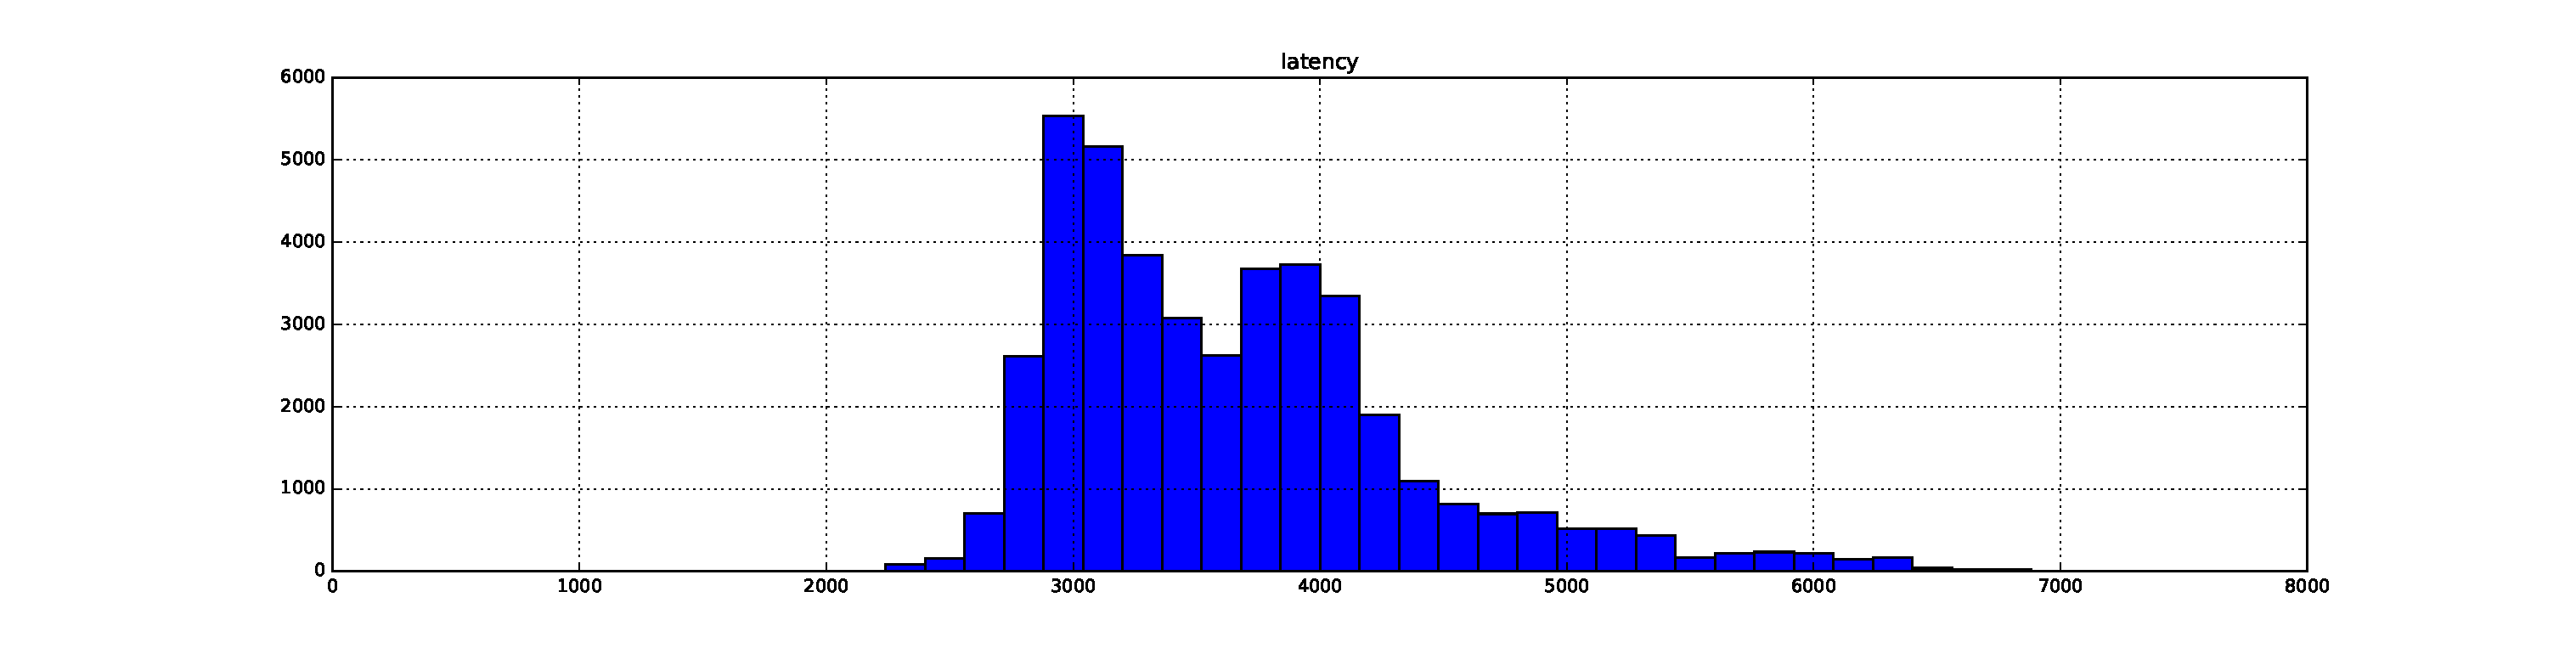
\includegraphics[width=\textwidth]{spark/3_4_1}
        \caption{3 Node latency histogram}
        \label{fig_yes_queue}
    \end{subfigure}
    ~ %add desired spacing between images, e. g. ~, \quad, \qquad, \hfill etc. 
    %(or a blank line to force the subfigure onto a new line)
    \begin{subfigure}[b]{0.49\textwidth}
        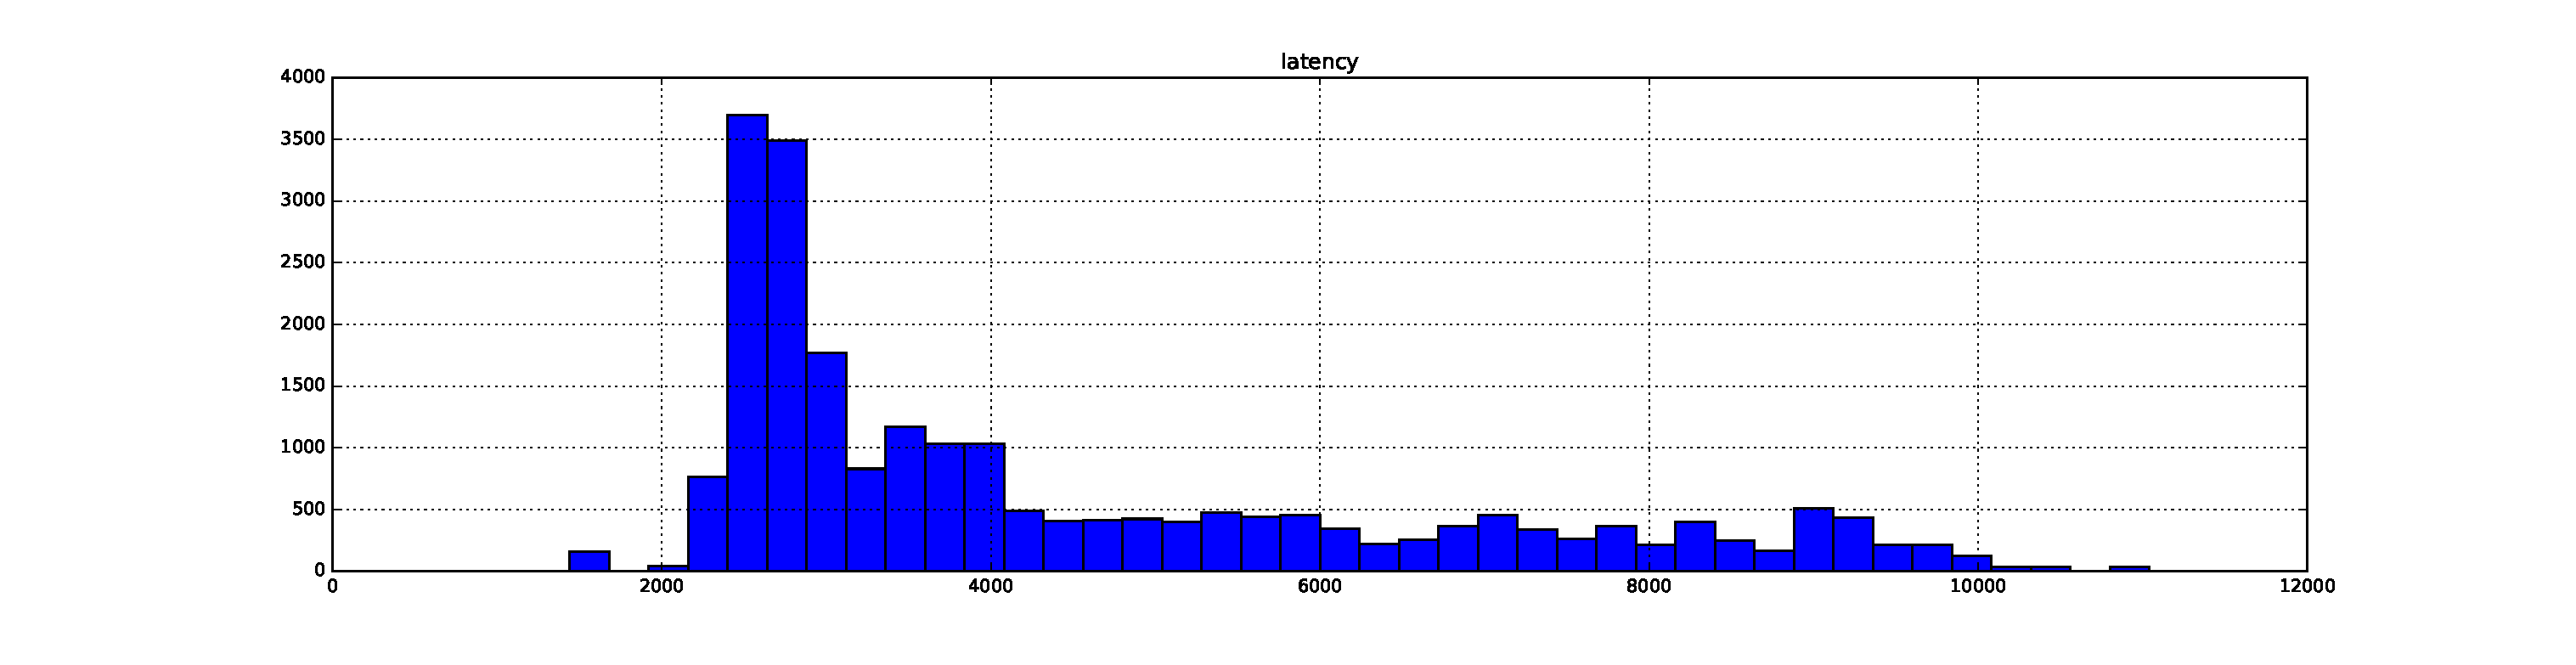
\includegraphics[width=\textwidth]{spark/4_4_1}
        \caption{4 Node latency histogram}
        \label{fig_partial_queue}
    \end{subfigure}
        \begin{subfigure}[b]{0.49\textwidth}
        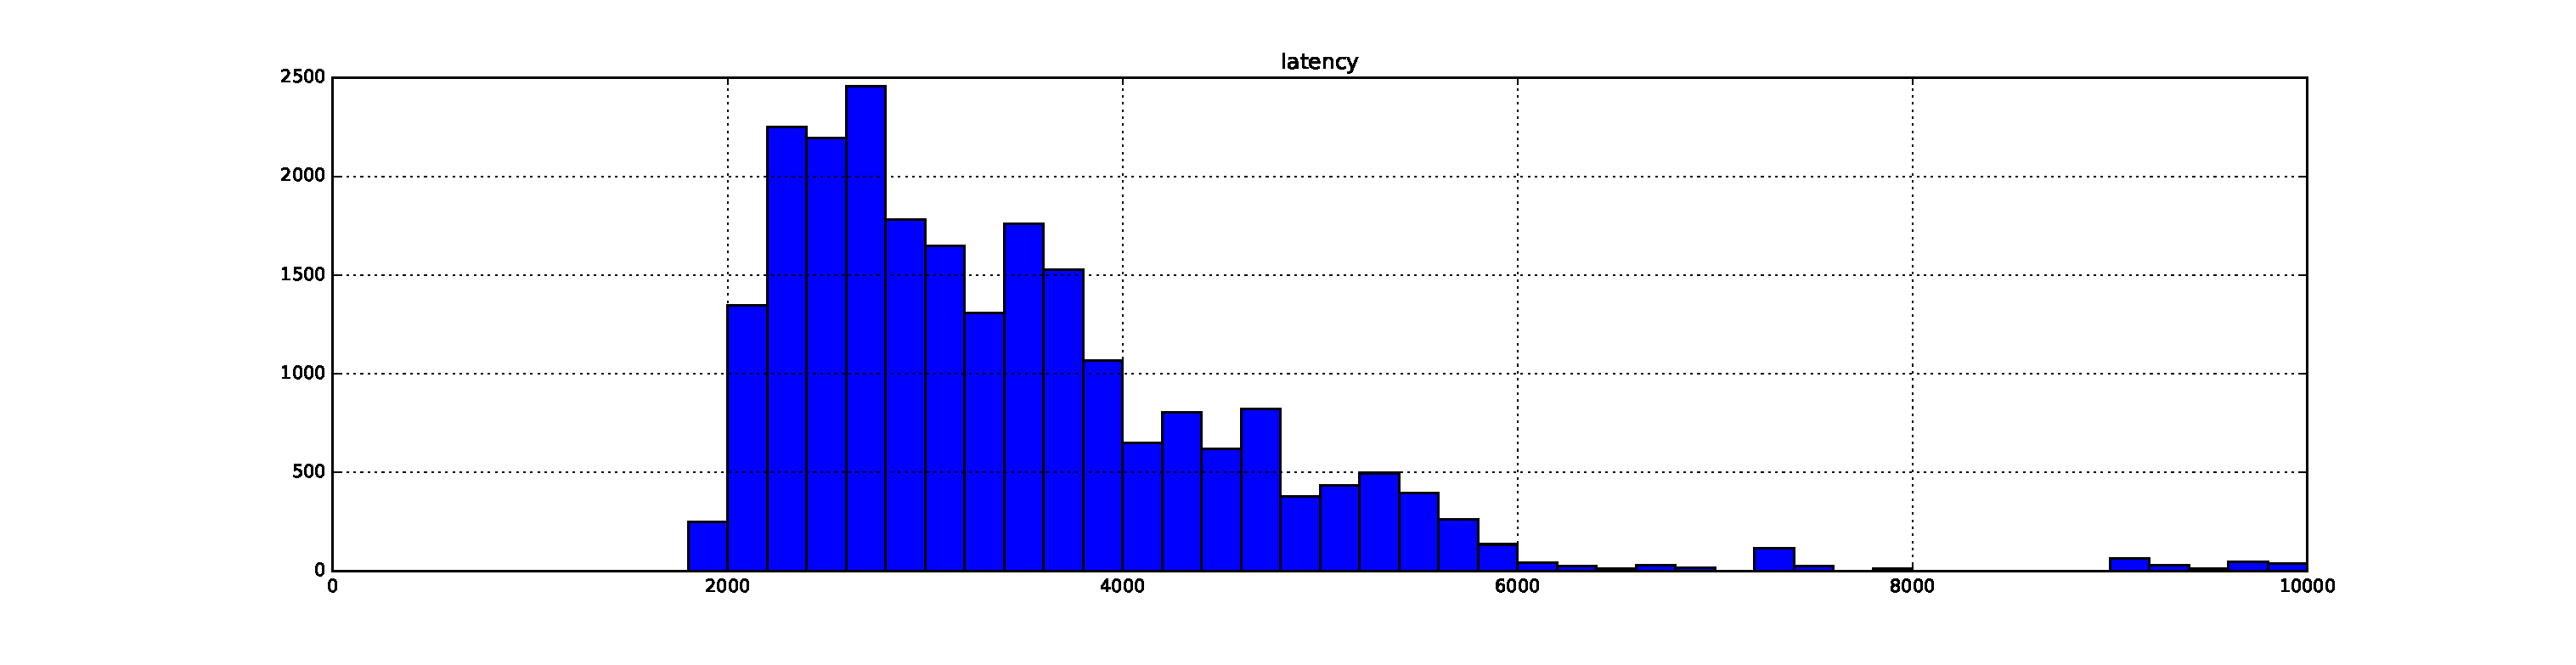
\includegraphics[width=\textwidth]{spark/8_4_1}
        \caption{8 Node latency histogram}
        \label{fig_partial_queue}
    \end{subfigure}


    \begin{subfigure}[b]{0.49\textwidth}
        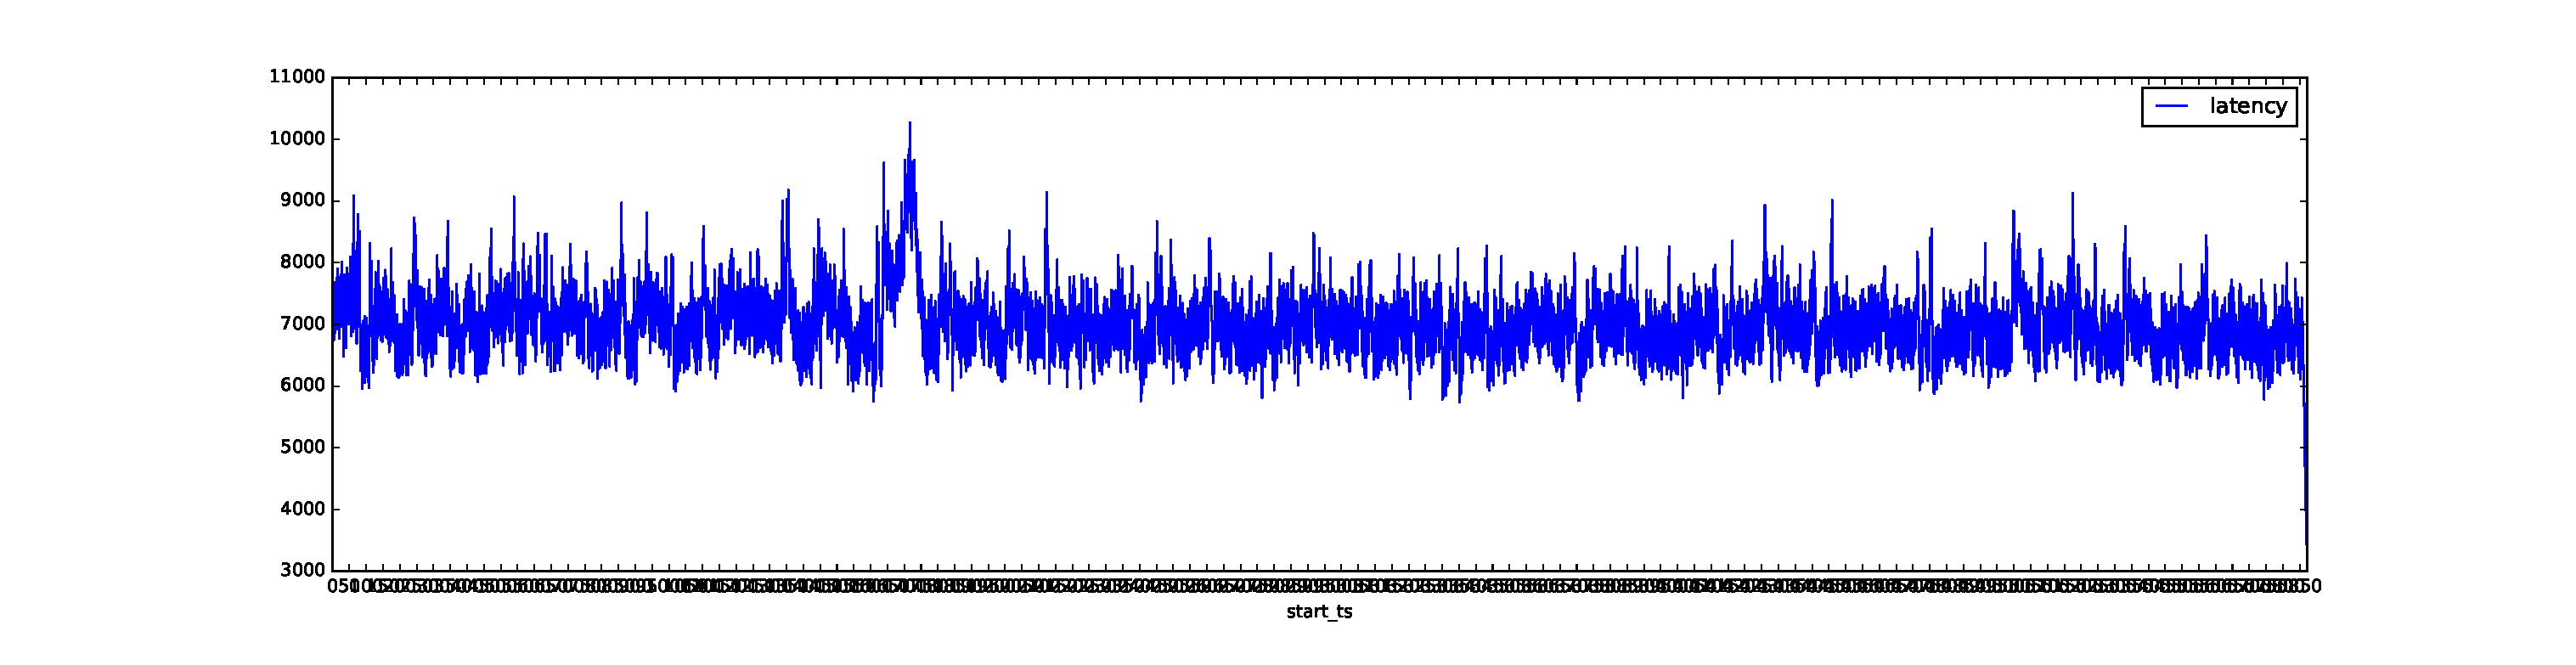
\includegraphics[width=\textwidth]{spark/2_4_2}
        \caption{2 Node latency time series}
        \label{fig_no_queue}
    \end{subfigure}
    ~ %add desired spacing between images, e. g. ~, \quad, \qquad, \hfill etc. 
      %(or a blank line to force the subfigure onto a new line)
    \begin{subfigure}[b]{0.49\textwidth}
        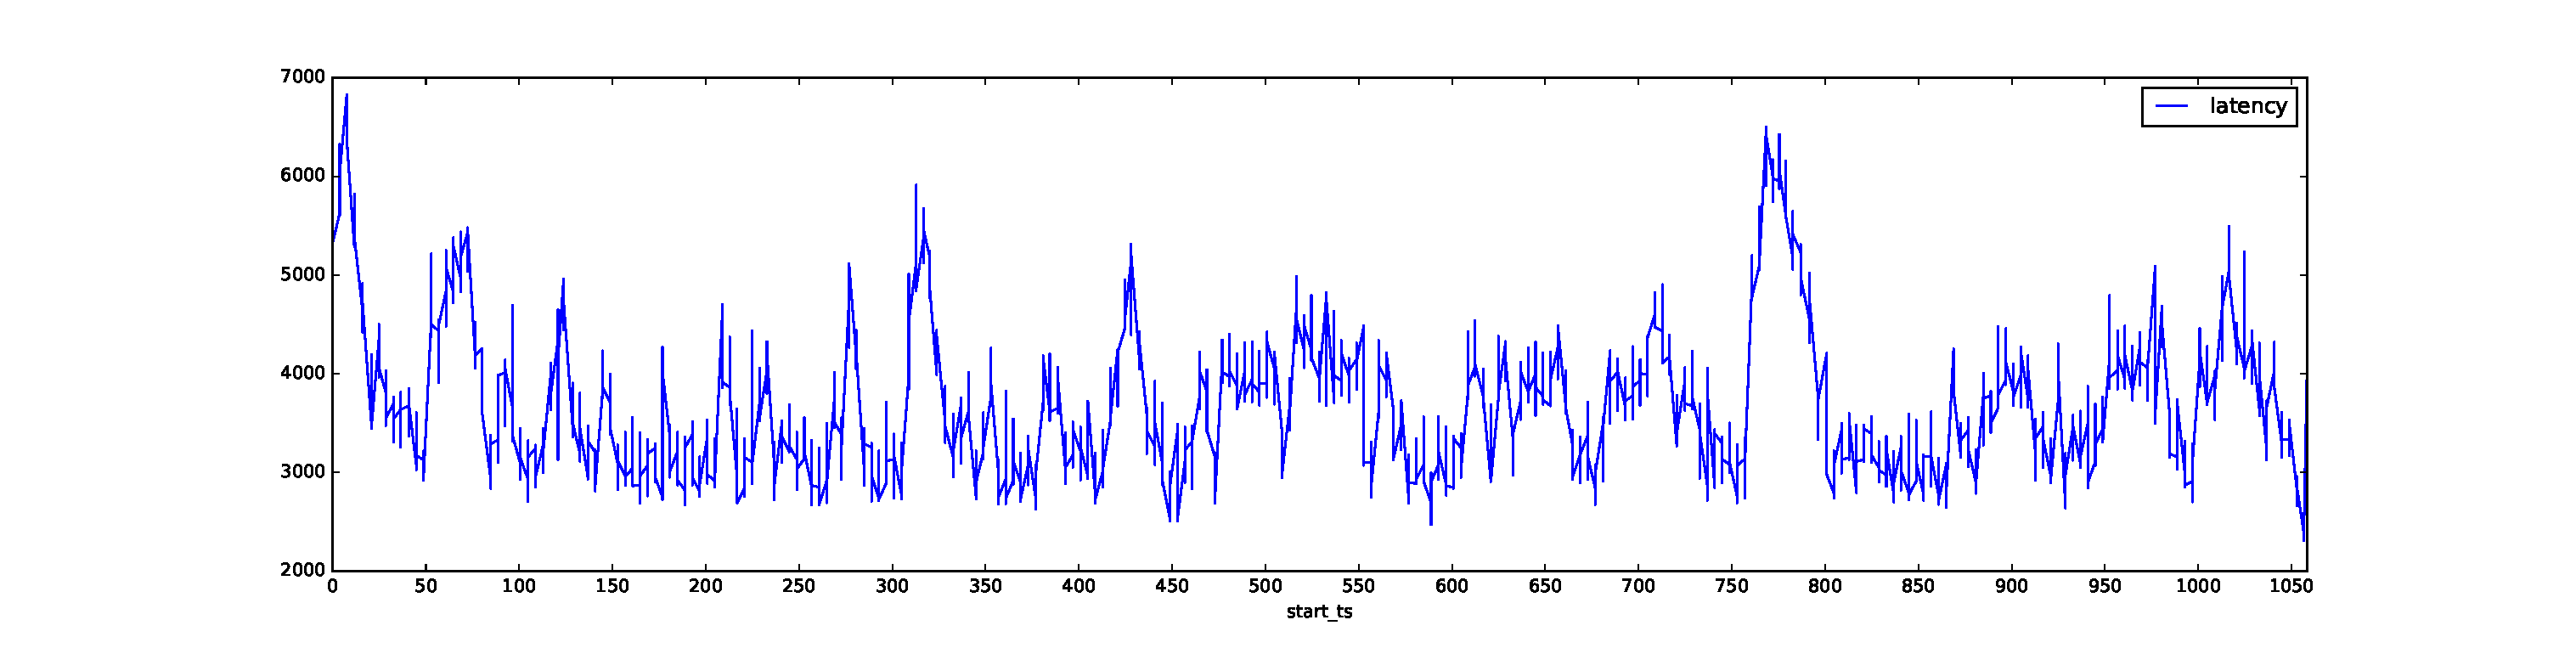
\includegraphics[width=\textwidth]{spark/3_4_2}
        \caption{3 Node latency time series}
        \label{fig_yes_queue}
    \end{subfigure}
    ~ %add desired spacing between images, e. g. ~, \quad, \qquad, \hfill etc. 
    %(or a blank line to force the subfigure onto a new line)
    \begin{subfigure}[b]{0.49\textwidth}
        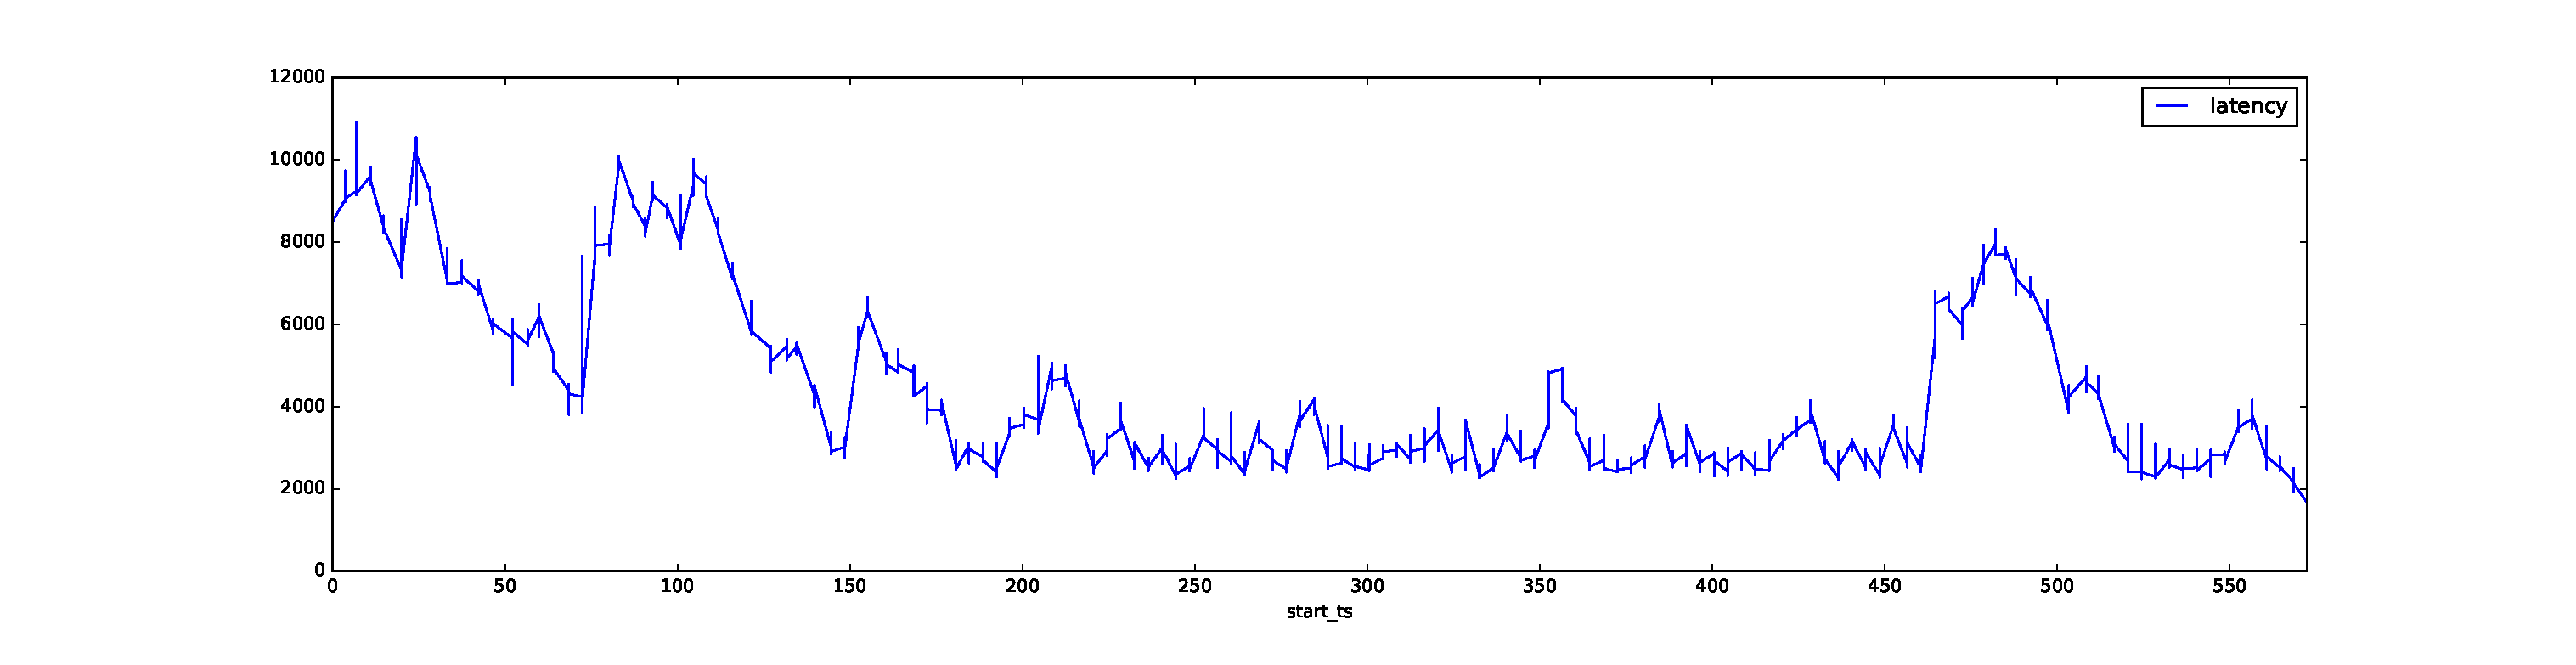
\includegraphics[width=\textwidth]{spark/4_4_2}
        \caption{4 Node latency time series}
        \label{fig_partial_queue}
    \end{subfigure}
        \begin{subfigure}[b]{0.49\textwidth}
        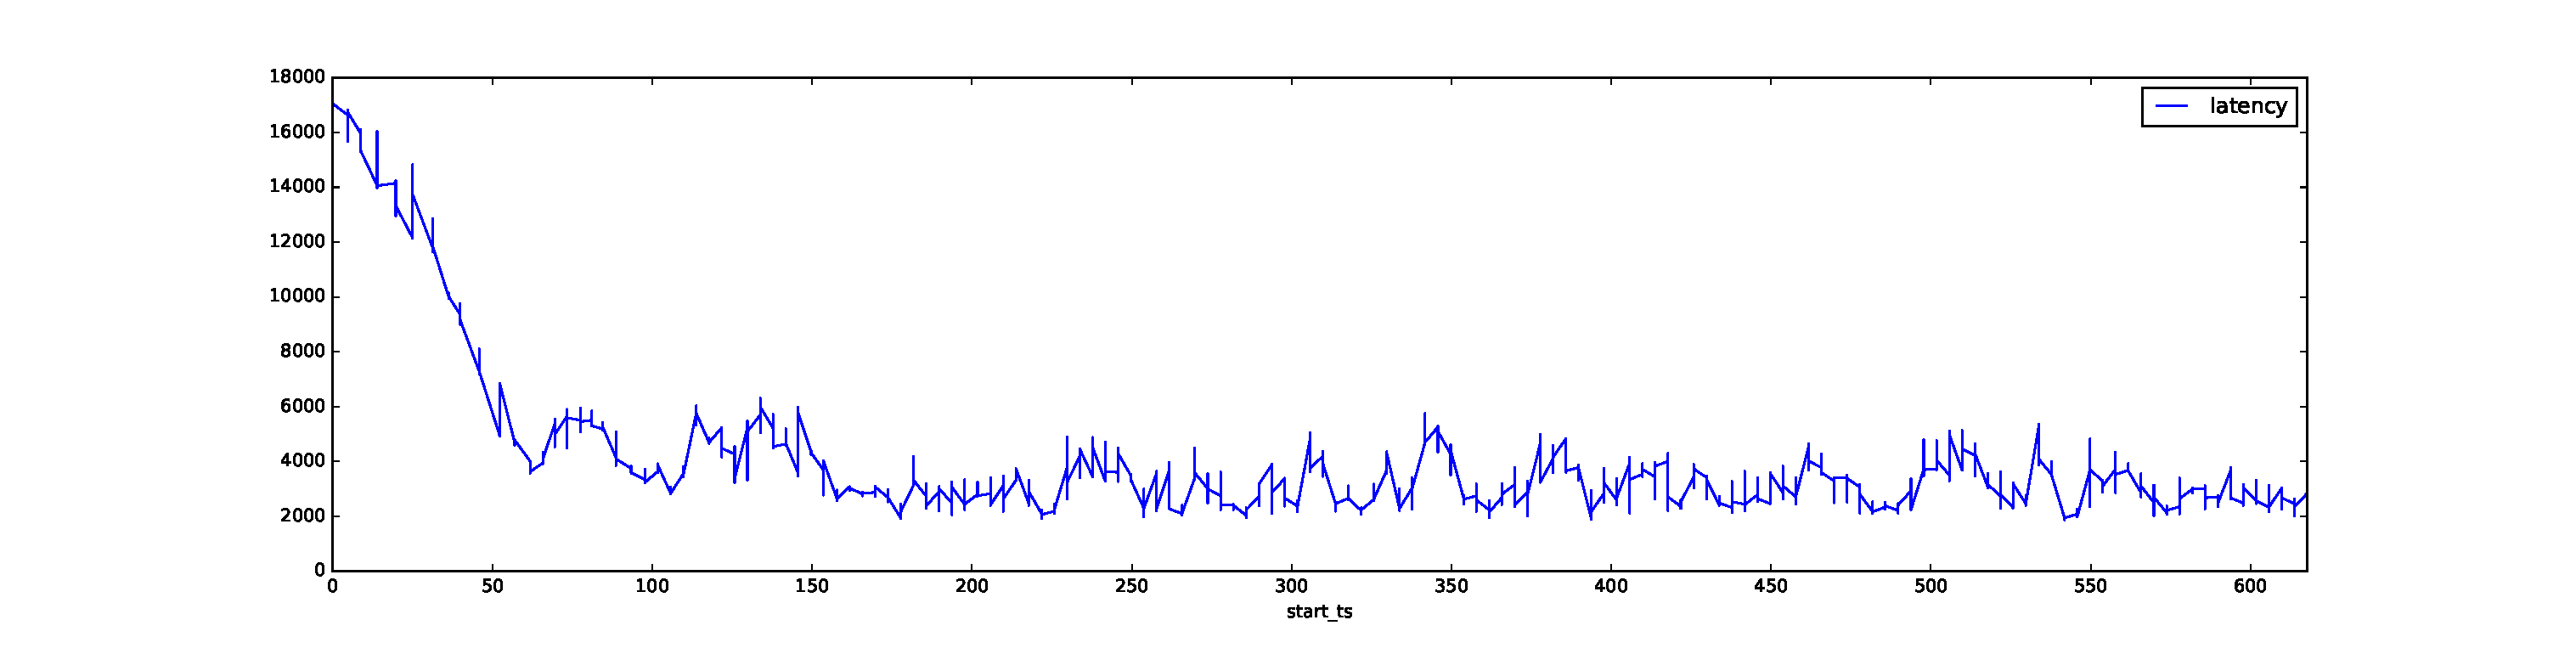
\includegraphics[width=\textwidth]{spark/8_4_2}
        \caption{8 Node latency time series}
        \label{fig_partial_queue}
    \end{subfigure}

    \label{fig_flink_agg_1}
        \caption{Latency of windowed aggregations for Spark (4 sec batch).}
\end{figure*}





\begin{figure*}
    \centering
    \begin{subfigure}[b]{0.49\textwidth}
        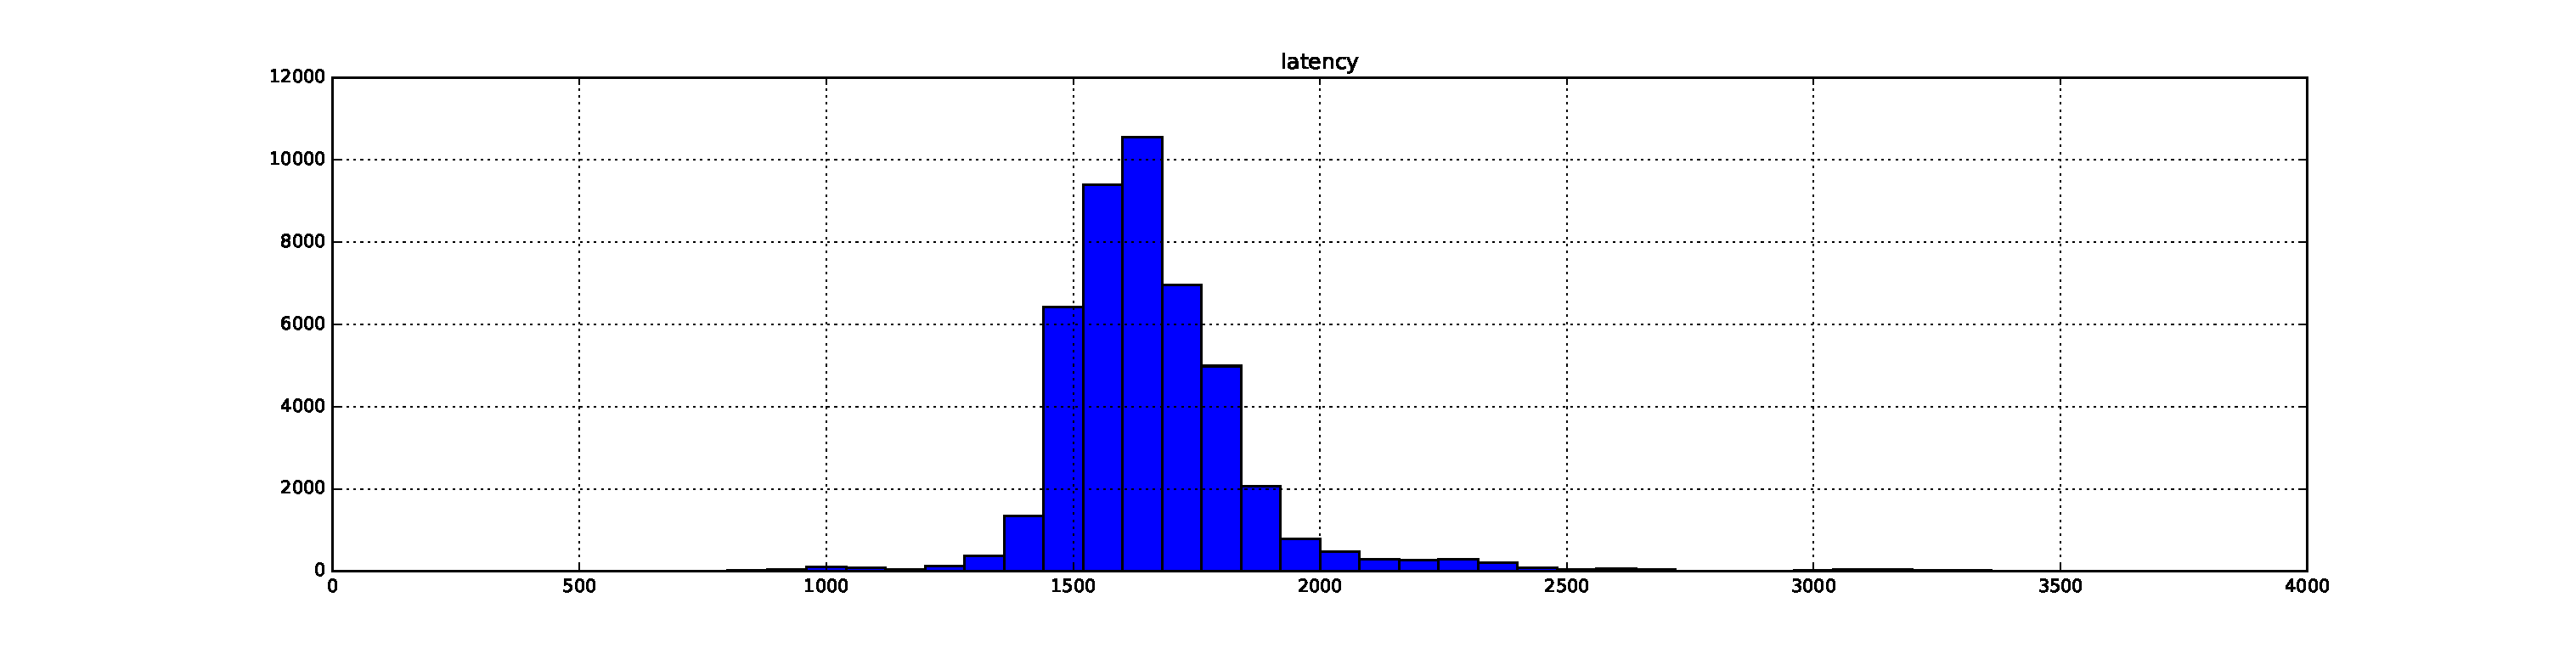
\includegraphics[width=\textwidth]{spark/2_2_1}
        \caption{2 Node latency histogram}
        \label{fig_no_queue}
    \end{subfigure}
    ~ %add desired spacing between images, e. g. ~, \quad, \qquad, \hfill etc. 
      %(or a blank line to force the subfigure onto a new line)
    \begin{subfigure}[b]{0.49\textwidth}
        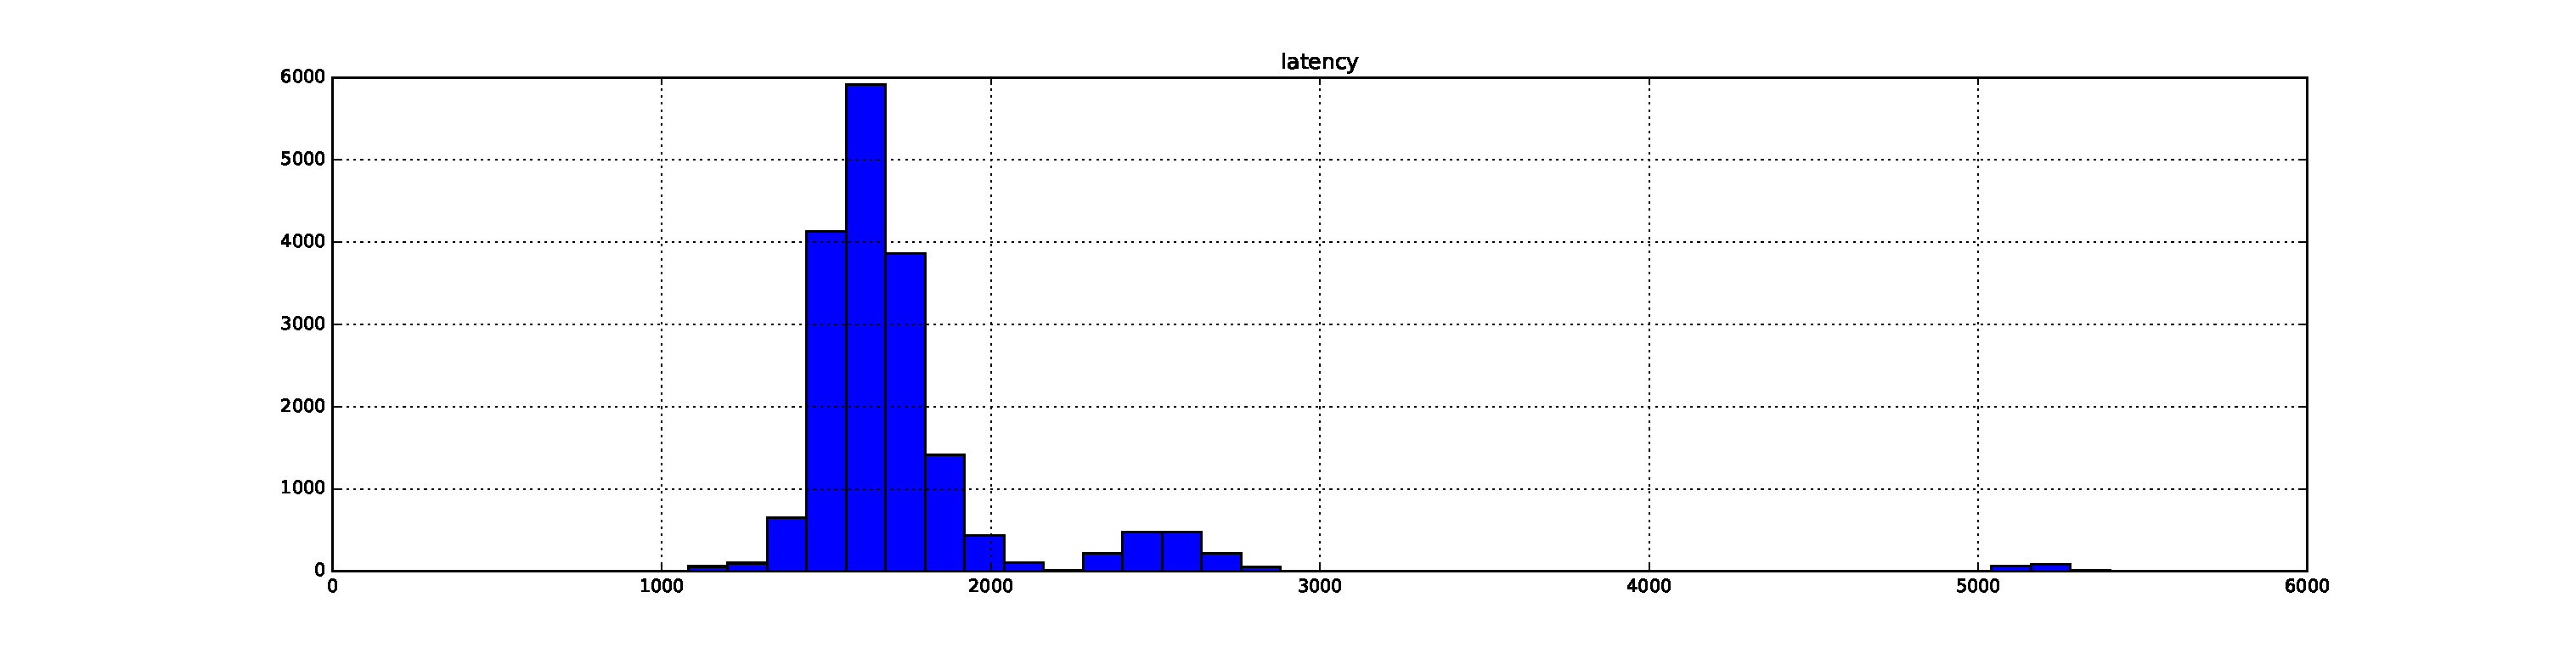
\includegraphics[width=\textwidth]{spark/3_2_1}
        \caption{3 Node latency histogram}
        \label{fig_yes_queue}
    \end{subfigure}
    ~ %add desired spacing between images, e. g. ~, \quad, \qquad, \hfill etc. 
    %(or a blank line to force the subfigure onto a new line)
    \begin{subfigure}[b]{0.49\textwidth}
        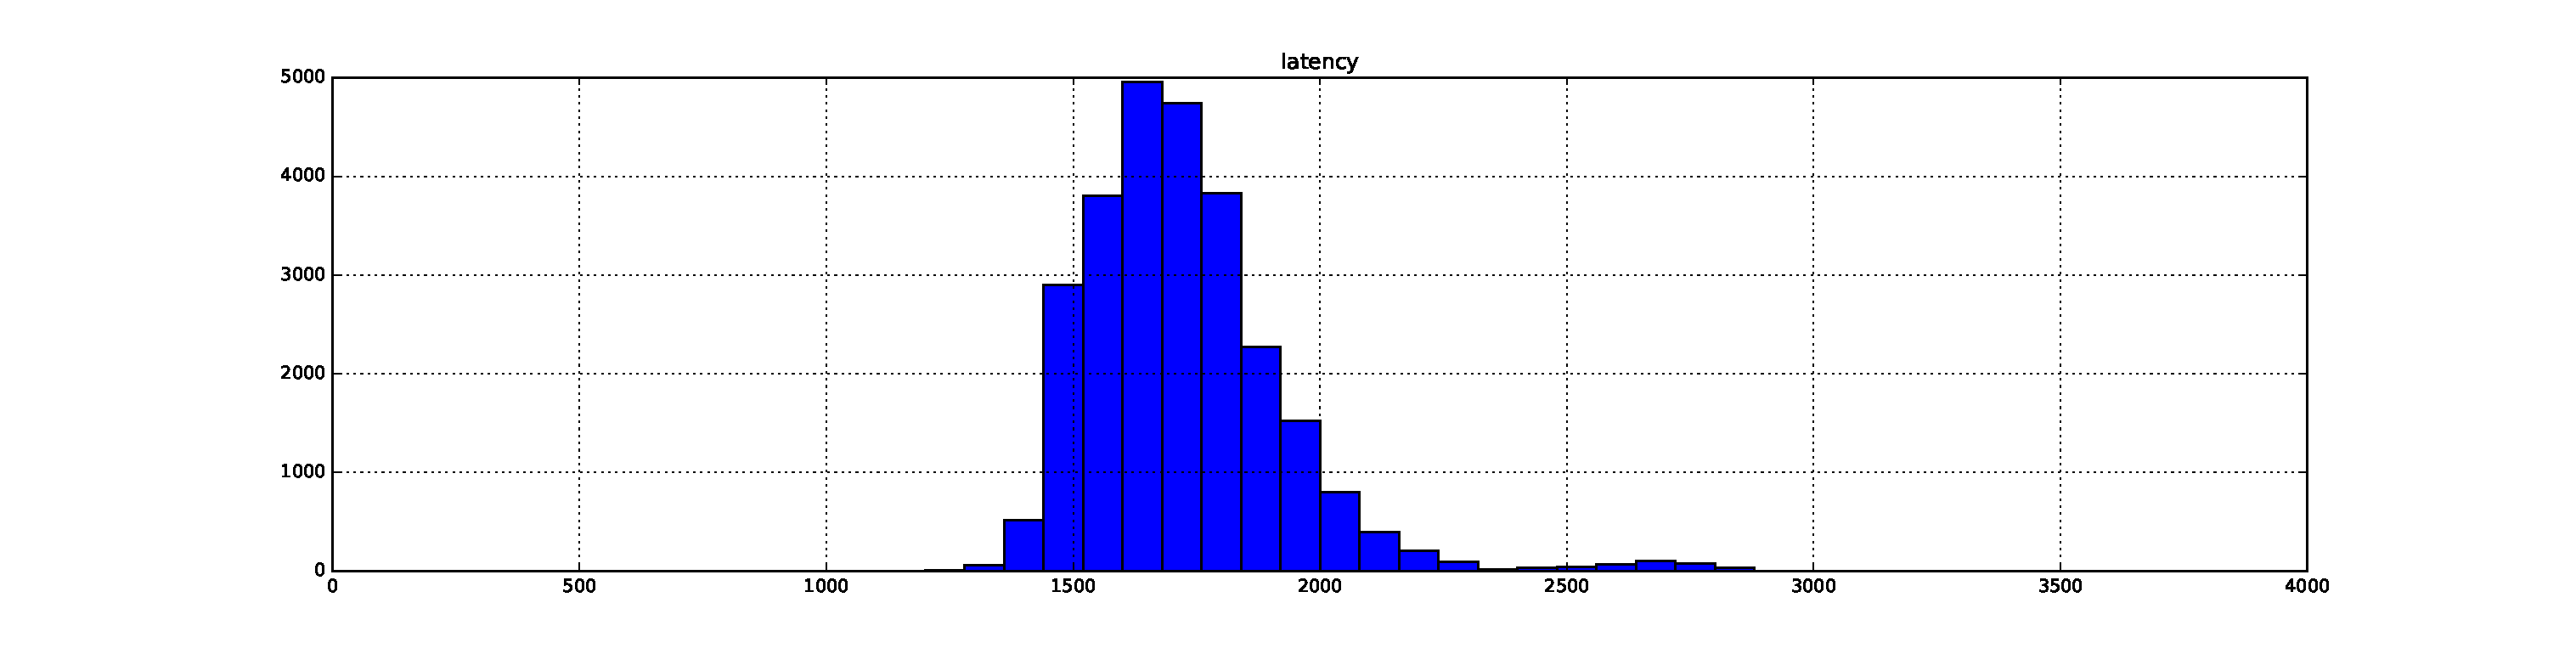
\includegraphics[width=\textwidth]{spark/4_2_1}
        \caption{4 Node latency histogram}
        \label{fig_partial_queue}
    \end{subfigure}
        \begin{subfigure}[b]{0.49\textwidth}
        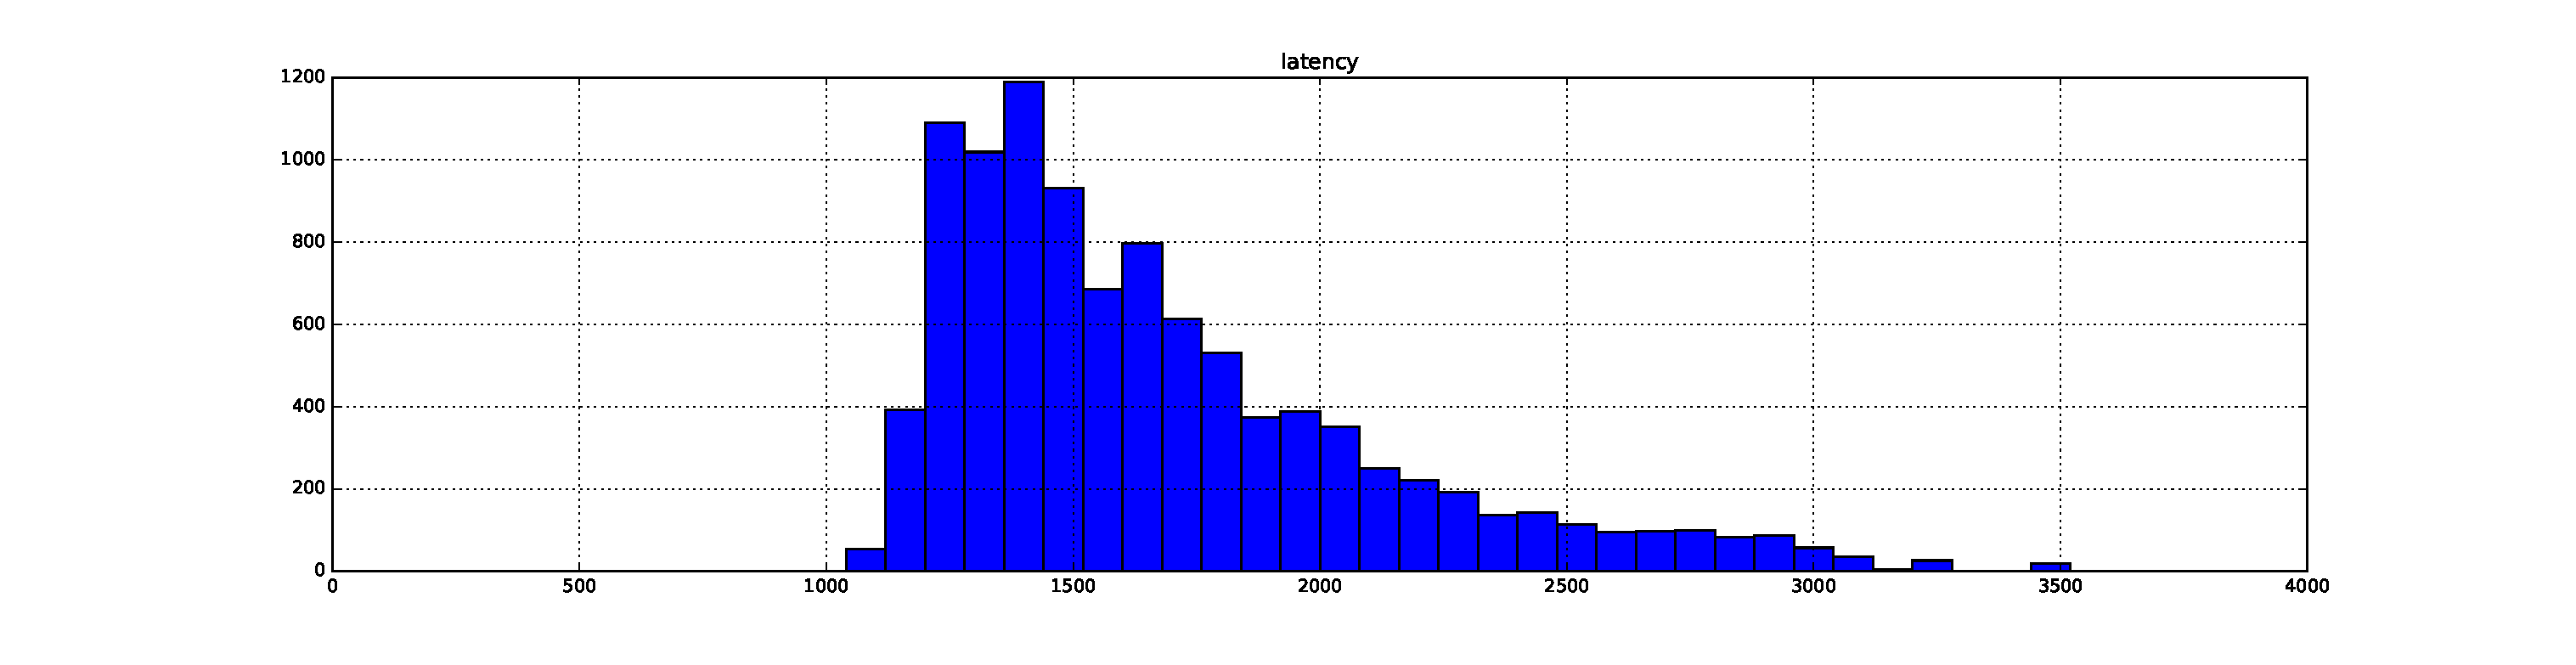
\includegraphics[width=\textwidth]{spark/8_2_1}
        \caption{8 Node latency histogram}
        \label{fig_partial_queue}
    \end{subfigure}


    \begin{subfigure}[b]{0.49\textwidth}
        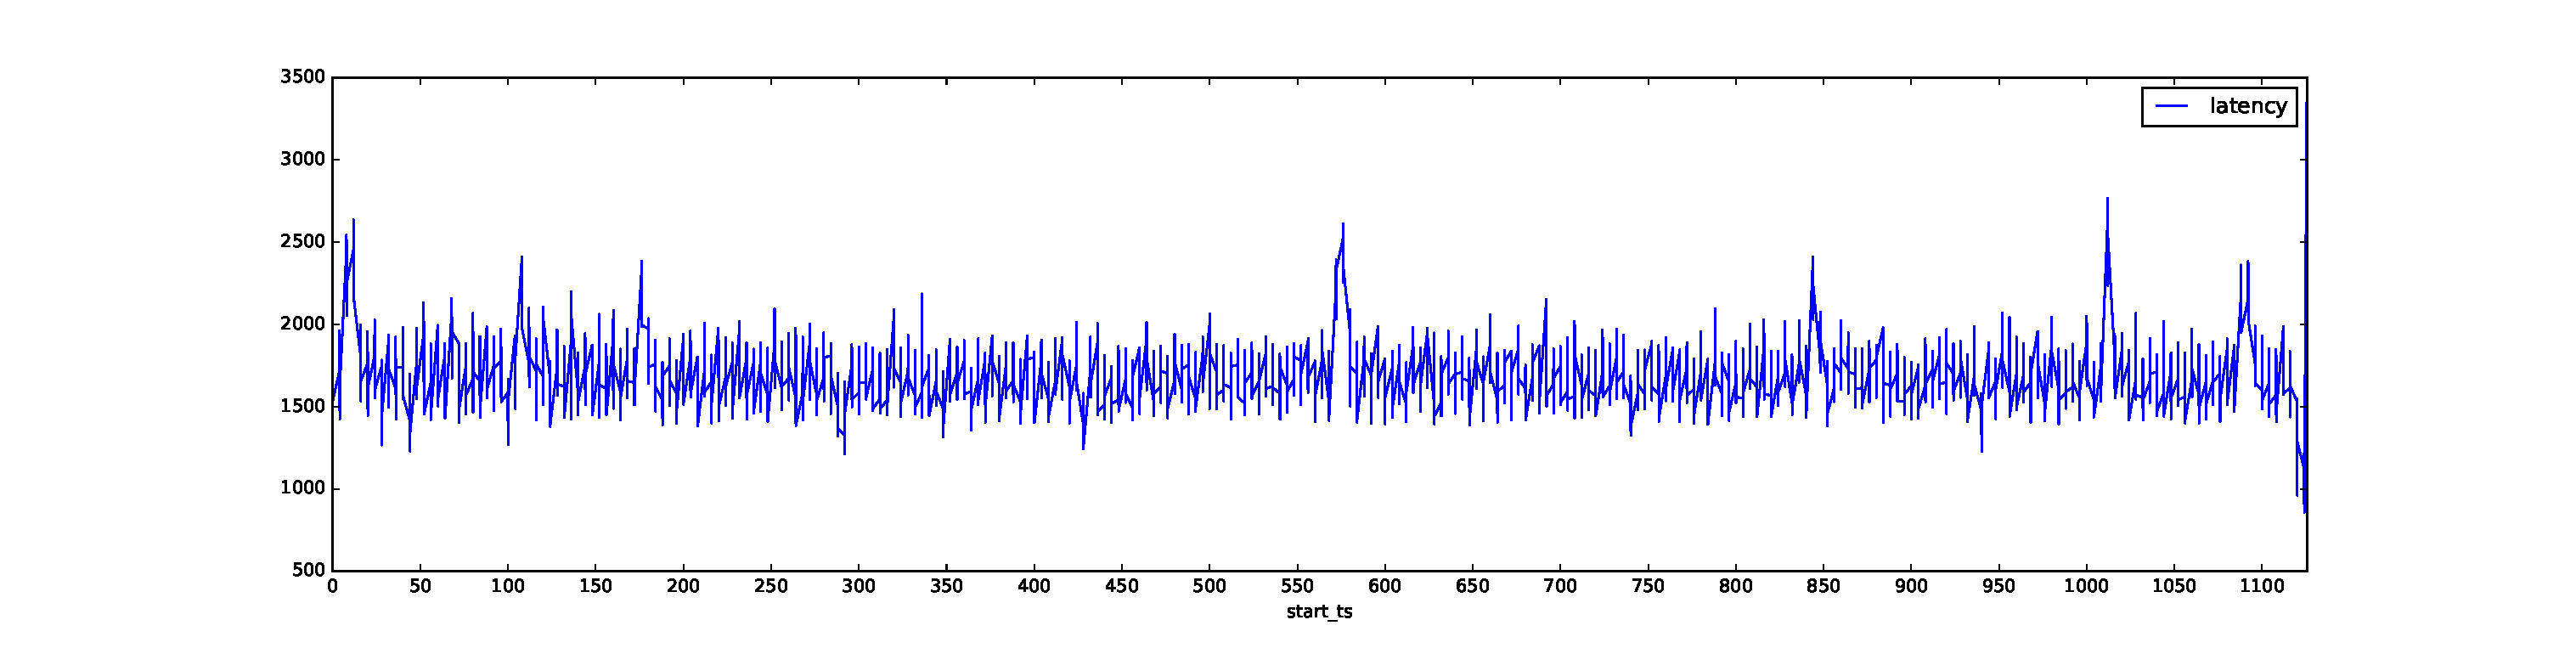
\includegraphics[width=\textwidth]{spark/2_2_2}
        \caption{2 Node latency time series}
        \label{fig_no_queue}
    \end{subfigure}
    ~ %add desired spacing between images, e. g. ~, \quad, \qquad, \hfill etc. 
      %(or a blank line to force the subfigure onto a new line)
    \begin{subfigure}[b]{0.49\textwidth}
        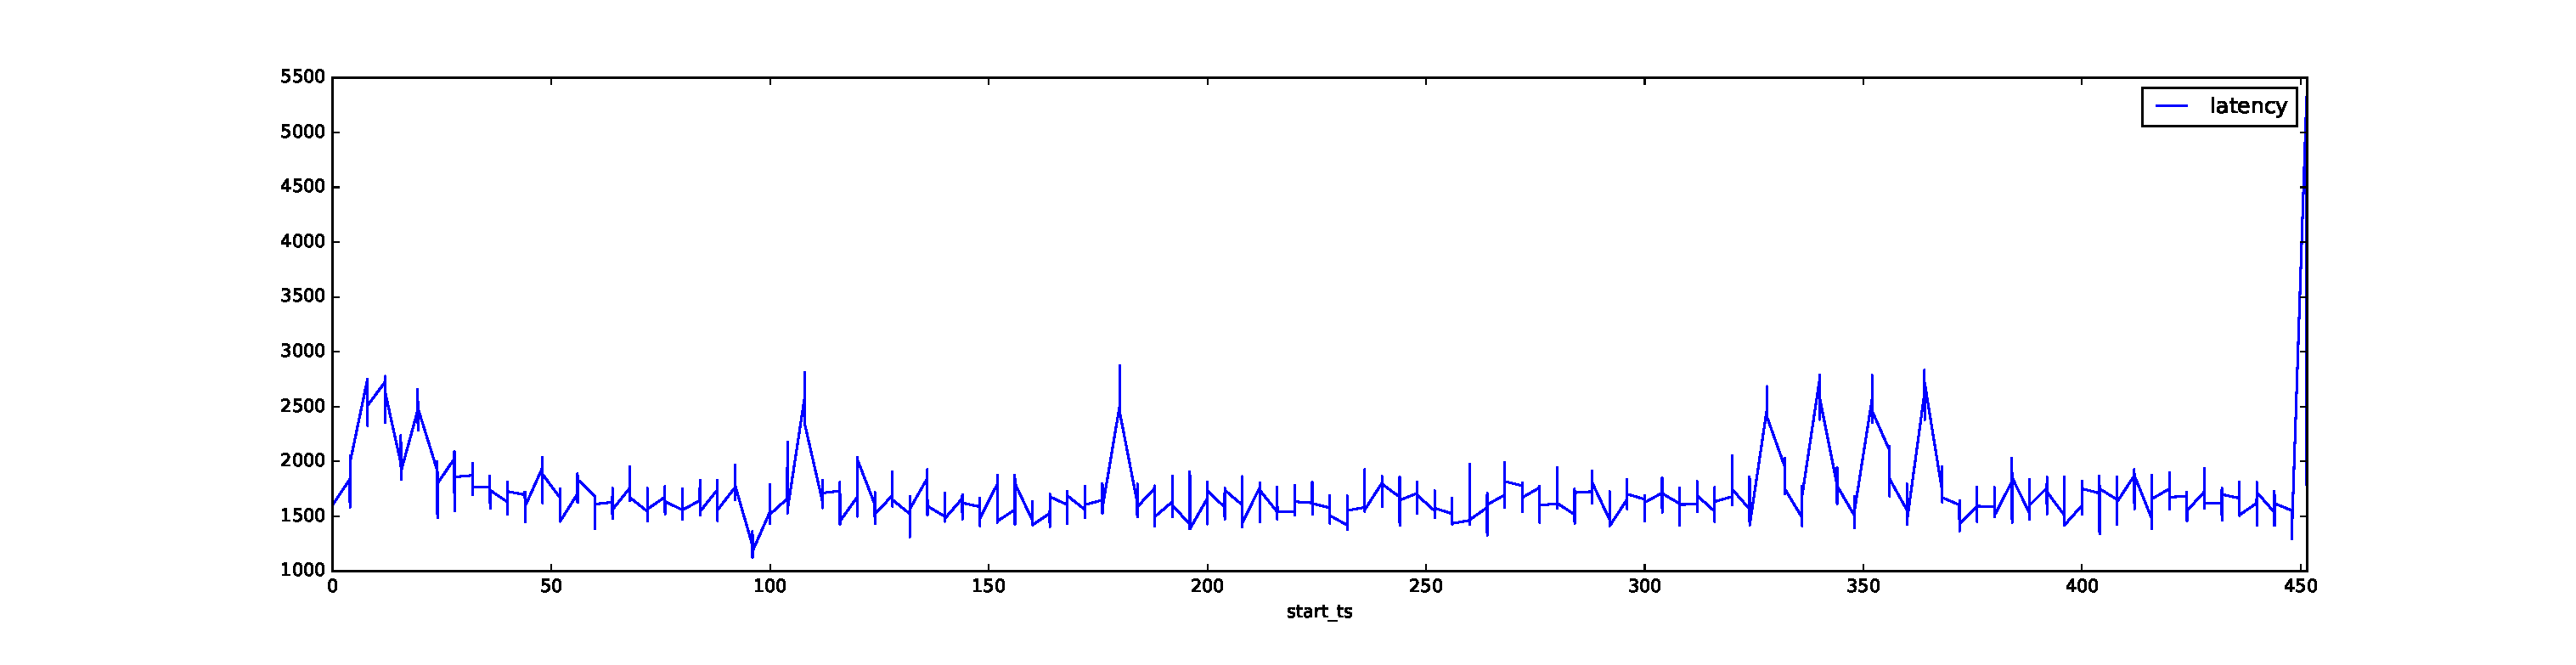
\includegraphics[width=\textwidth]{spark/3_2_2}
        \caption{3 Node latency time series}
        \label{fig_yes_queue}
    \end{subfigure}
    ~ %add desired spacing between images, e. g. ~, \quad, \qquad, \hfill etc. 
    %(or a blank line to force the subfigure onto a new line)
    \begin{subfigure}[b]{0.49\textwidth}
        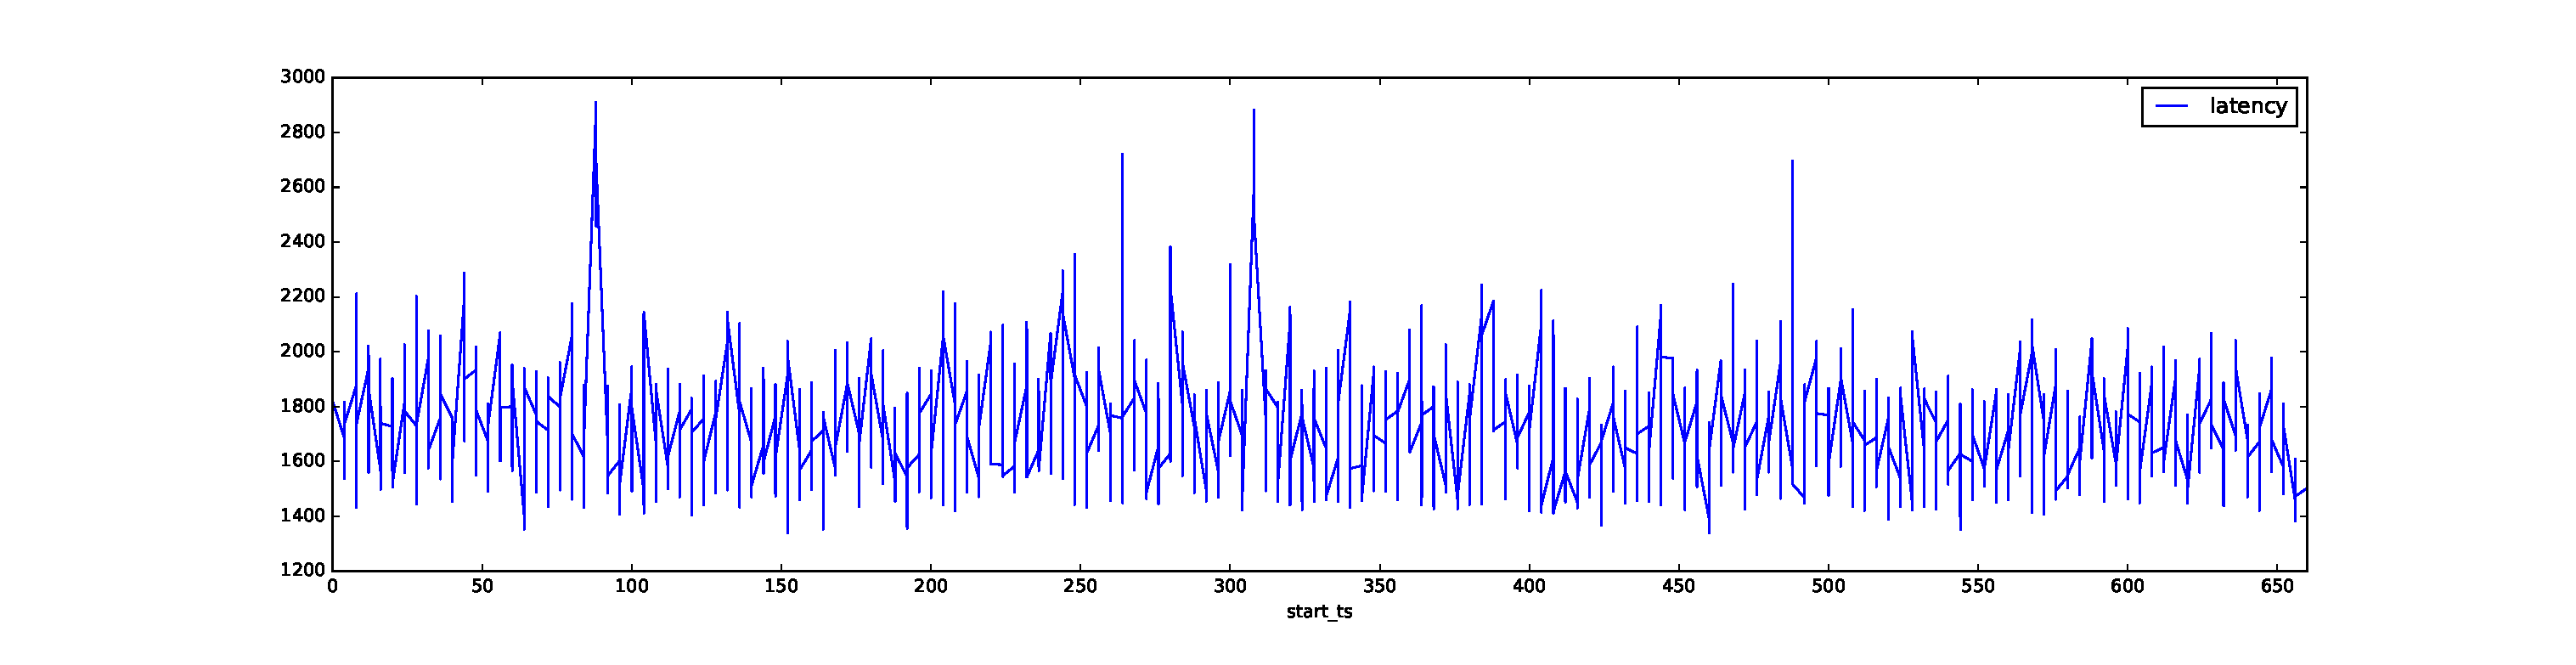
\includegraphics[width=\textwidth]{spark/4_2_2}
        \caption{4 Node latency time series}
        \label{fig_partial_queue}
    \end{subfigure}
        \begin{subfigure}[b]{0.49\textwidth}
        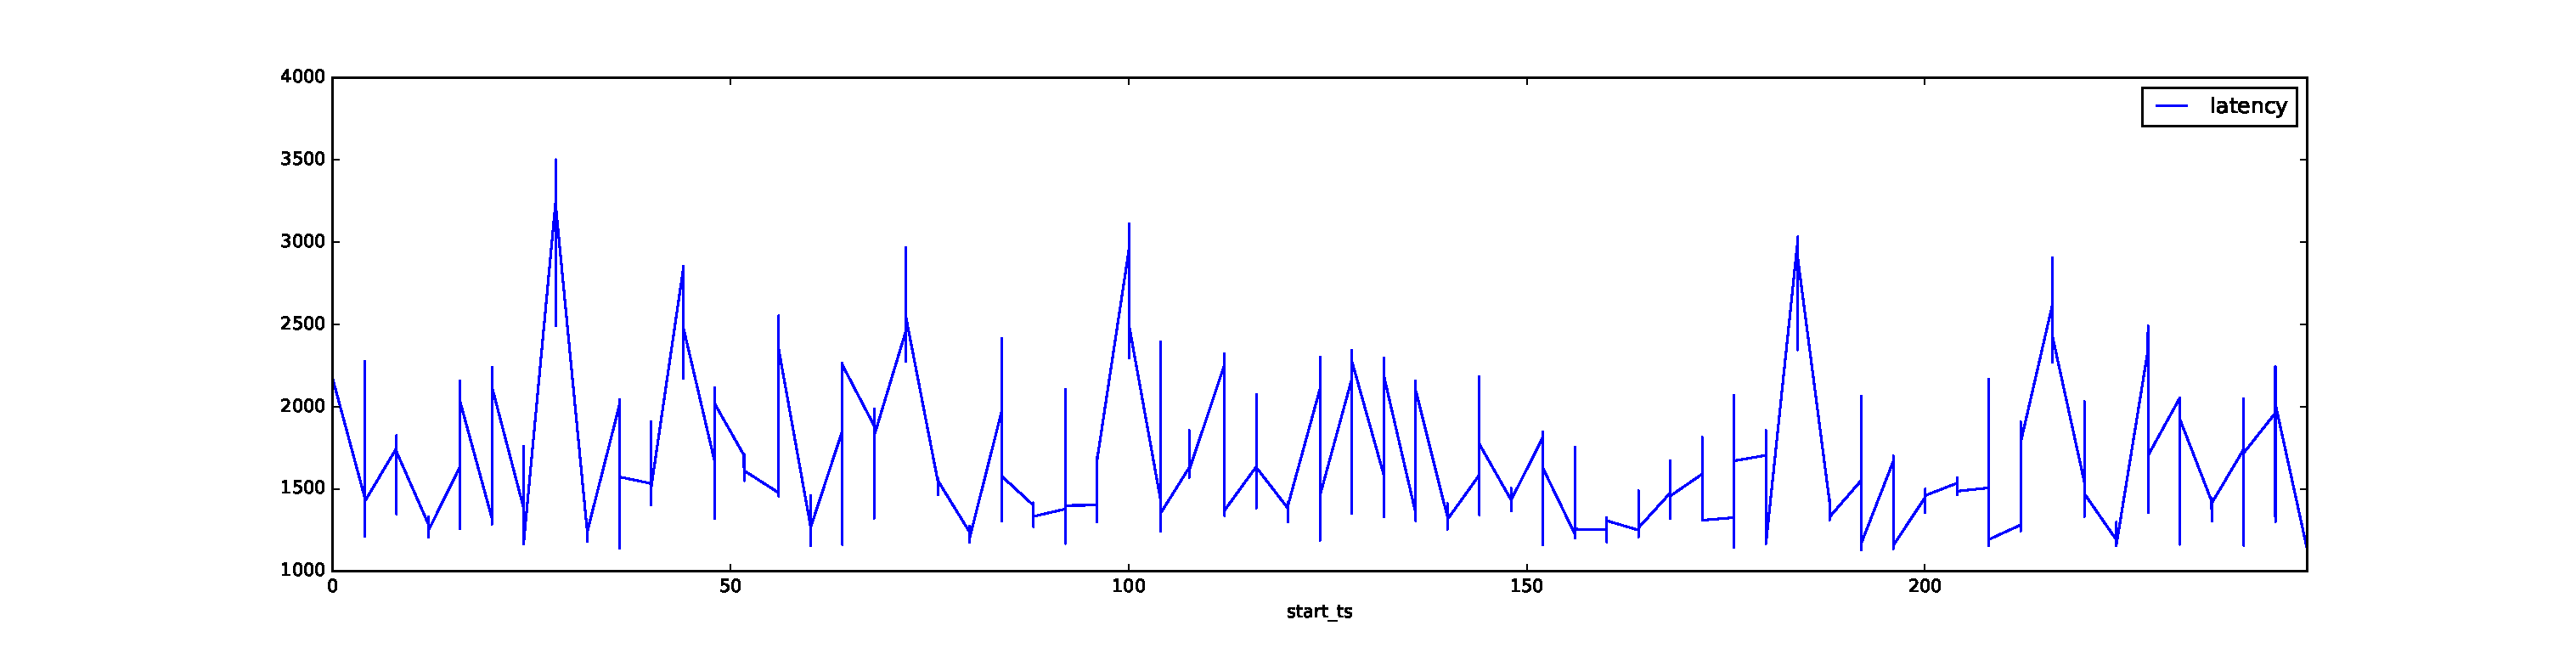
\includegraphics[width=\textwidth]{spark/8_2_2}
        \caption{8 Node latency time series}
        \label{fig_partial_queue}
    \end{subfigure}

    \label{fig_flink_agg_1}
        \caption{Latency of windowed aggregations for Spark (2 sec batch).}
\end{figure*}





\subsubsection{Flink}





\begin{figure*}
    \centering
    \begin{subfigure}[b]{0.49\textwidth}
        \includegraphics[width=\textwidth]{flink/2_1}
        \caption{2 Node latency histogram}
        \label{fig_no_queue}
    \end{subfigure}
    ~ %add desired spacing between images, e. g. ~, \quad, \qquad, \hfill etc. 
      %(or a blank line to force the subfigure onto a new line)
    \begin{subfigure}[b]{0.49\textwidth}
        \includegraphics[width=\textwidth]{flink/3_1}
        \caption{3 Node latency histogram}
        \label{fig_yes_queue}
    \end{subfigure}
    ~ %add desired spacing between images, e. g. ~, \quad, \qquad, \hfill etc. 
    %(or a blank line to force the subfigure onto a new line)
    \begin{subfigure}[b]{0.49\textwidth}
        \includegraphics[width=\textwidth]{flink/4_1}
        \caption{4 Node latency histogram}
        \label{fig_partial_queue}
    \end{subfigure}
        \begin{subfigure}[b]{0.49\textwidth}
        \includegraphics[width=\textwidth]{flink/8_1}
        \caption{8 Node latency histogram}
        \label{fig_partial_queue}
    \end{subfigure}


    \begin{subfigure}[b]{0.49\textwidth}
        \includegraphics[width=\textwidth]{flink/2_2}
        \caption{2 Node latency time series}
        \label{fig_no_queue}
    \end{subfigure}
    ~ %add desired spacing between images, e. g. ~, \quad, \qquad, \hfill etc. 
      %(or a blank line to force the subfigure onto a new line)
    \begin{subfigure}[b]{0.49\textwidth}
        \includegraphics[width=\textwidth]{flink/3_2}
        \caption{3 Node latency time series}
        \label{fig_yes_queue}
    \end{subfigure}
    ~ %add desired spacing between images, e. g. ~, \quad, \qquad, \hfill etc. 
    %(or a blank line to force the subfigure onto a new line)
    \begin{subfigure}[b]{0.49\textwidth}
        \includegraphics[width=\textwidth]{flink/4_2}
        \caption{4 Node latency time series}
        \label{fig_partial_queue}
    \end{subfigure}
        \begin{subfigure}[b]{0.49\textwidth}
        \includegraphics[width=\textwidth]{flink/8_2}
        \caption{8 Node latency time series}
        \label{fig_partial_queue}
    \end{subfigure}

    \label{fig_flink_agg_1}
        \caption{Latency of windowed aggregations for Flink.}
\end{figure*}


    \begin{table}
        \begin{tabular}{lllll}\toprule
            &\textbf{2 Node} & \textbf{3 Node} & \textbf{4 Node} & \textbf{8 Node}\\\midrule
            Storm & 345 & 235 & 345 & 345\\
            Spark(2sec) & 8K & 15K & 23K & 23K\\
            Spark(4sec) & 240K & 480K & 656K & 920K\\
            Flink & 1072K & 1232K & 1232K & 1232K\\
            \\\bottomrule
        \end{tabular}
        \caption{Sustainable throughput for windowed aggregations}\label{Tab1}
    \end{table} 

    \begin{table}
        \begin{tabular}{lllll}\toprule
            &\textbf{2 Node} & \textbf{3 Node} & \textbf{4 Node} & \textbf{8 Node}\\\midrule
            Storm & 345 & 235 & 345 & 345\\
            Spark(2sec) & 376 & 707 & 1.1K & 1.1K\\
            Spark(4sec) & 12K & 24K & 33K & 47K\\
            Flink & 53K & 58K & 58K & 58K\\
            \\\bottomrule
        \end{tabular}
        \caption{Average Window size for windowed aggregations}\label{Tab1}
    \end{table} 

    \begin{table}
        \begin{tabular}{lllll}\toprule
            &\textbf{2 Node} & \textbf{3 Node} & \textbf{4 Node} & \textbf{8 Node}\\\midrule
            Storm & 345 & 235 & 345 & 345\\
            Spark(2sec) & 1.6s & 1.7s & 1.7s & 1.6s\\
            Spark(4sec) & 6.9s & 3.6s & 4.4s & 3.9s\\
            Flink & 0.3s & 0.4s & 0.35s & 0.28s\\
            \\\bottomrule
        \end{tabular}
        \caption{Average Latency for windowed aggregations}\label{Tab1}
    \end{table} 


    \begin{table}
        \begin{tabular}{lllll}\toprule
            &\textbf{2 Node} & \textbf{3 Node} & \textbf{4 Node} & \textbf{8 Node}\\\midrule
            Storm & NULL & NULL & NULL & NULL\\
            Spark(2sec) & NULL & NULL & NULL & NULL\\
            Spark(4sec) & NULL & NULL & NULL & NULL\\
            Flink & 528K & 587K & 643K & 806K\\
            \\\bottomrule
        \end{tabular}
        \caption{Sustainable throughput for windowed joins}\label{Tab1}
    \end{table} 


    \begin{table}
        \begin{tabular}{lllll}\toprule
            &\textbf{2 Node} & \textbf{3 Node} & \textbf{4 Node} & \textbf{8 Node}\\\midrule
            Storm & NULL & NULL & NULL & NULL\\
            Spark(2sec) & NULL & NULL & NULL & NULL\\
            Spark(4sec) & NULL & NULL & NULL & NULL\\
            Flink & 3.6s & 4.7s & 4s & 3.4\\
            \\\bottomrule
        \end{tabular}
        \caption{Average Latency for windowed joins}\label{Tab1}
    \end{table} 


\subsection{Joins}





\begin{figure*}
    \centering
    \begin{subfigure}[b]{0.49\textwidth}
        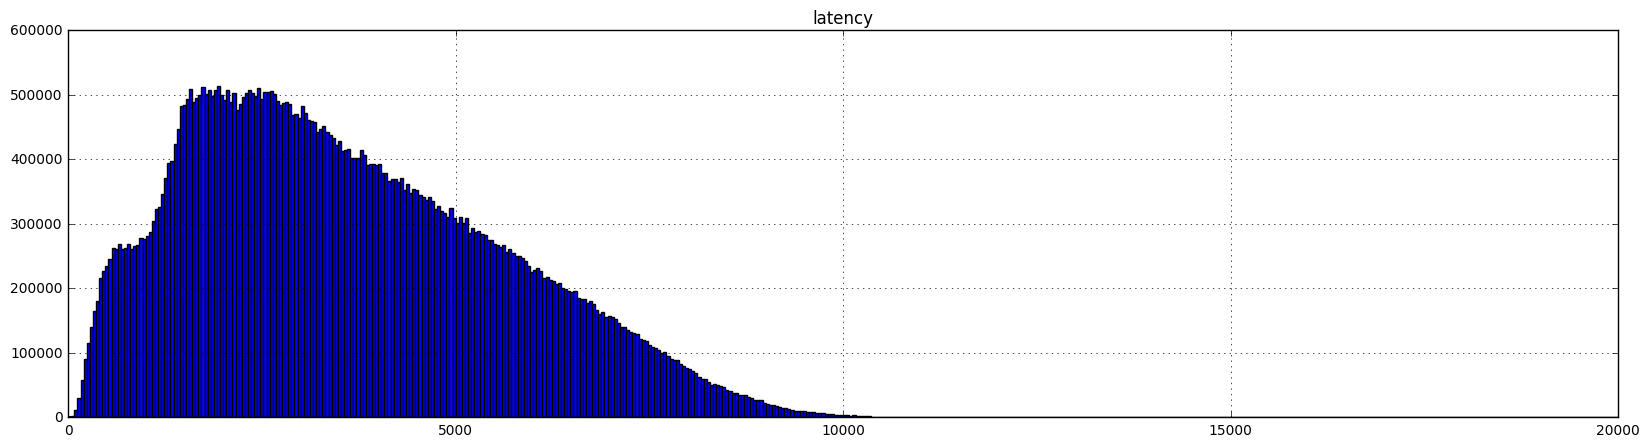
\includegraphics[width=\textwidth]{join/flink/2}
        \caption{2 Node latency histogram}
        \label{fig_no_queue}
    \end{subfigure}
    ~ %add desired spacing between images, e. g. ~, \quad, \qquad, \hfill etc. 
      %(or a blank line to force the subfigure onto a new line)
    \begin{subfigure}[b]{0.49\textwidth}
        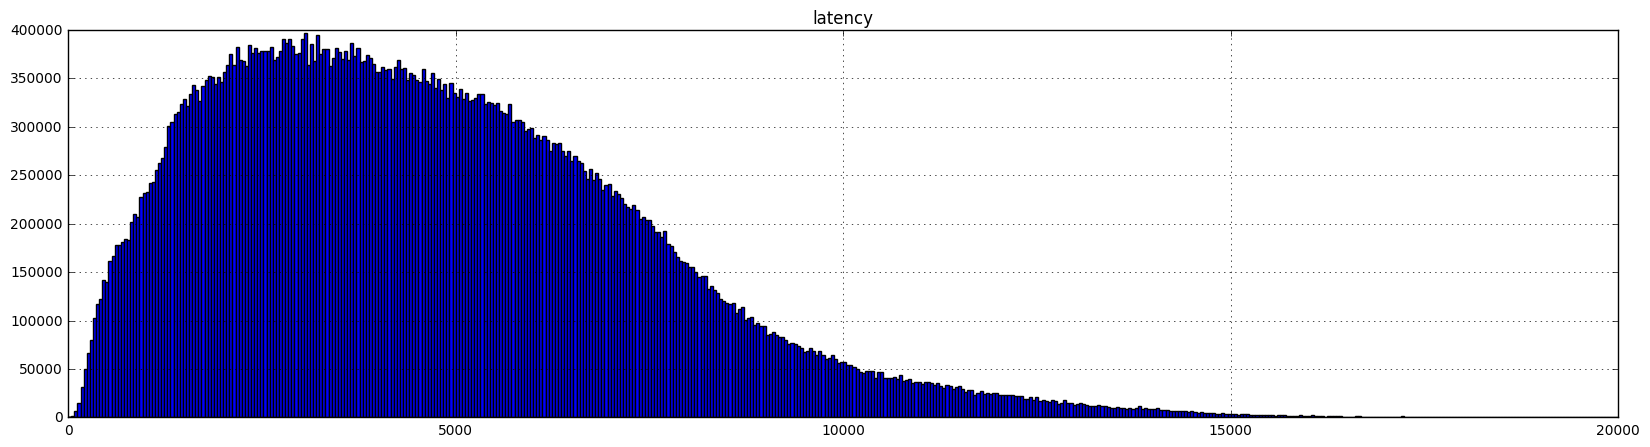
\includegraphics[width=\textwidth]{join/flink/3}
        \caption{3 Node latency histogram}
        \label{fig_yes_queue}
    \end{subfigure}
    ~ %add desired spacing between images, e. g. ~, \quad, \qquad, \hfill etc. 
    %(or a blank line to force the subfigure onto a new line)
    \begin{subfigure}[b]{0.49\textwidth}
        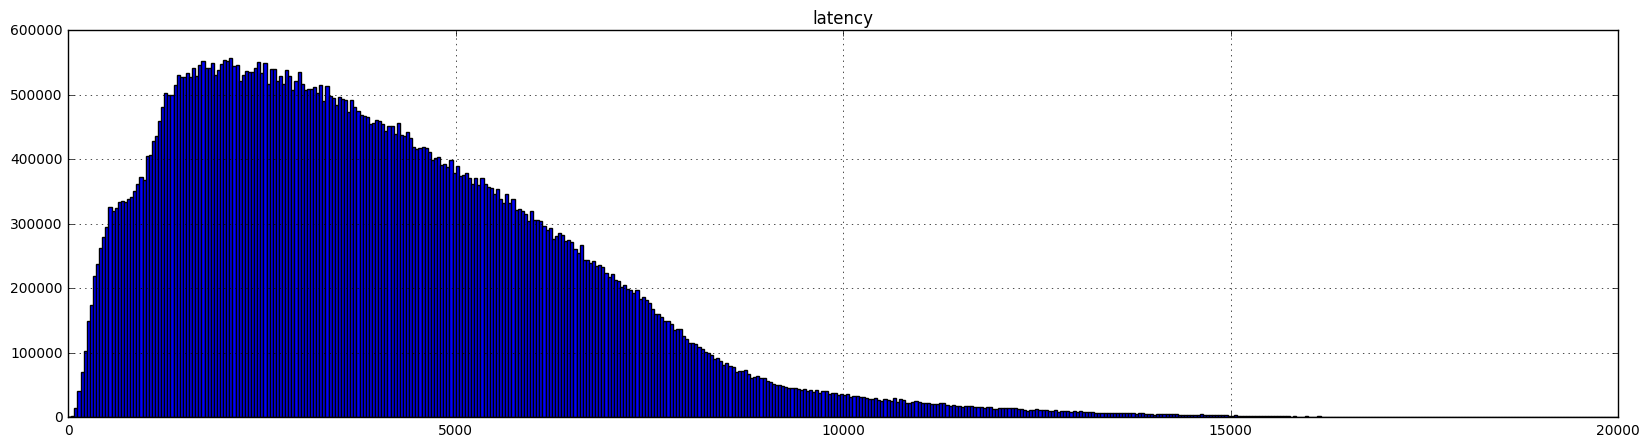
\includegraphics[width=\textwidth]{join/flink/4}
        \caption{4 Node latency histogram}
        \label{fig_partial_queue}
    \end{subfigure}
        \begin{subfigure}[b]{0.49\textwidth}
        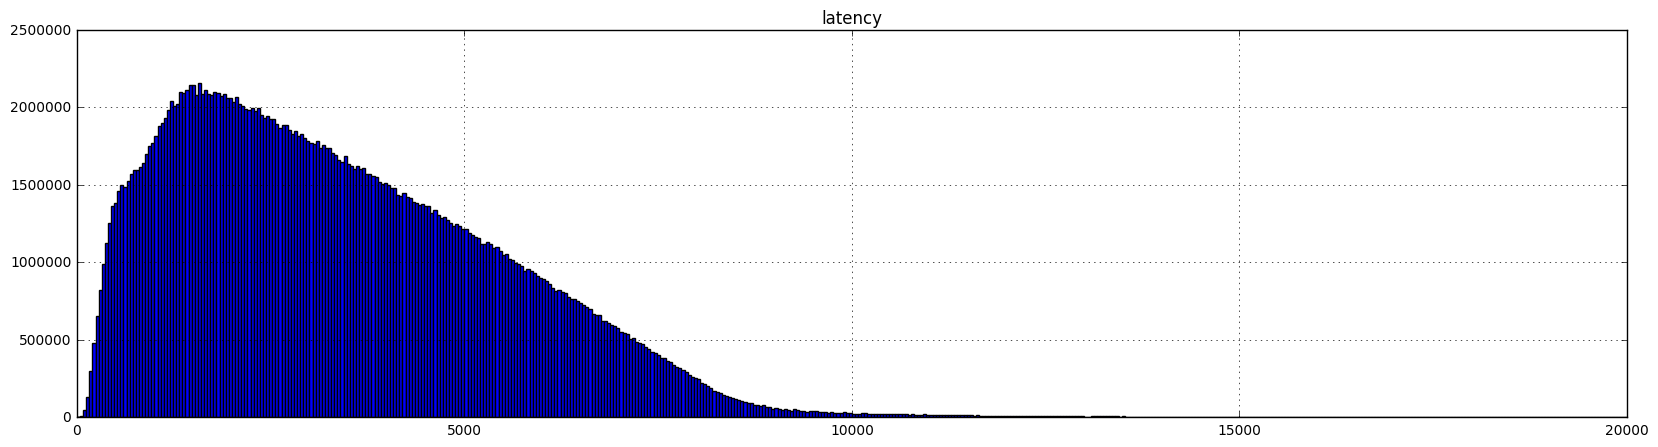
\includegraphics[width=\textwidth]{join/flink/8}
        \caption{8 Node latency histogram}
        \label{fig_partial_queue}
    \end{subfigure}



    \label{fig_flink_agg_1}
        \caption{Latency of windowed joins for Flink.}
\end{figure*}
